\chapter{To verify truth table for XOR gate}

\section{Apparatus}
%\label{sec:objectives}
	\begin{itemize}
		\tightlist
		\item Kit for realization of gates
		\item Connecting Leads
	\end{itemize}

\section{Theory}
	The 'Exclusive-OR' gate is a circuit which will give a high output if either, but not both of its two inputs are high. An encircled plus sign ($\oplus$) is used to show the Ex-OR operation.
	\begin{figure}[h]
		\centering
		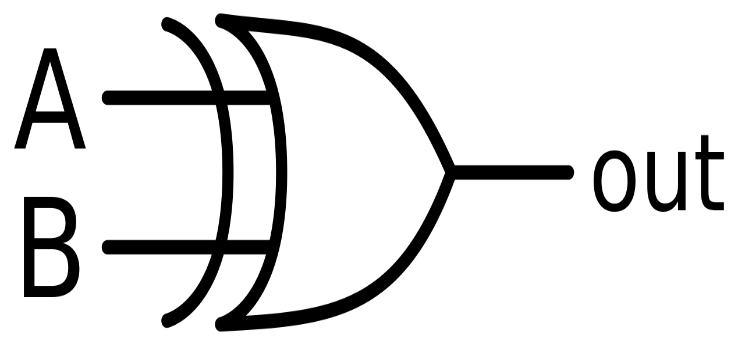
\includegraphics{img/exp6/1}
		\caption{Symbol for XOR gate}
		\label{fig:6:1}
	\end{figure}
	\begin{figure}[h]
		\centering
		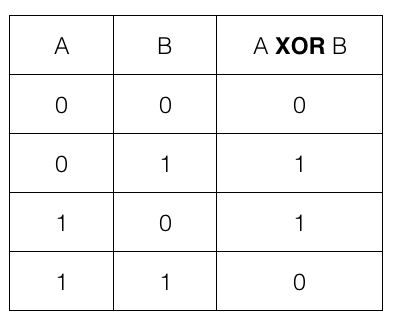
\includegraphics{img/exp6/2}
		\caption{Truth Table for XOR gate}
		\label{fig:6:2}
	\end{figure}
	
	Ex-OR gate is created from AND, NAND and OR gates.The output is high only when both the inputs are different.
	
	\begin{figure}[h]
		\centering
		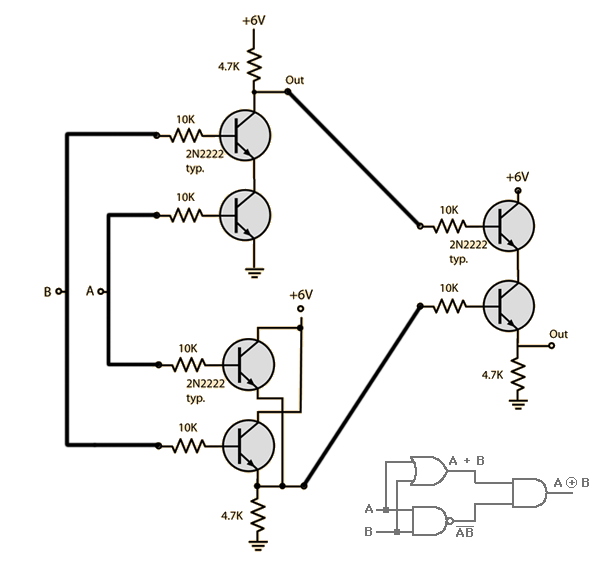
\includegraphics{img/exp6/3}
		\caption{Circut for making XOR gate}
		\label{fig:6:3}
	\end{figure}
				
\section{Procedure}
	\subsubsection{Simulator 1}
	\begin{itemize}
		\tightlist
		\item Connect the supply(+5V) to the circuit.
		\item Press the switches for inputs "A" and "B".
		\item The bulb glows if one of the switches is ON and one of the switches is OFF else it won't glow.
		\item Repeat step-2 and step-3 for all state of inputs.
	\end{itemize}

	\subsubsection{Simulator 2}
	\begin{itemize}
		\tightlist
		\item Enter the Boolean input "A" and "B".
		\item Enter the Boolean output for your corresponding inputs.
		\item Click on "Check" Button to verify your output.
		\item Click "Print" if you want to get print out of Truth Table.
	\end{itemize}


\section{Observations}
	\begin{figure}[h]
		\centering
		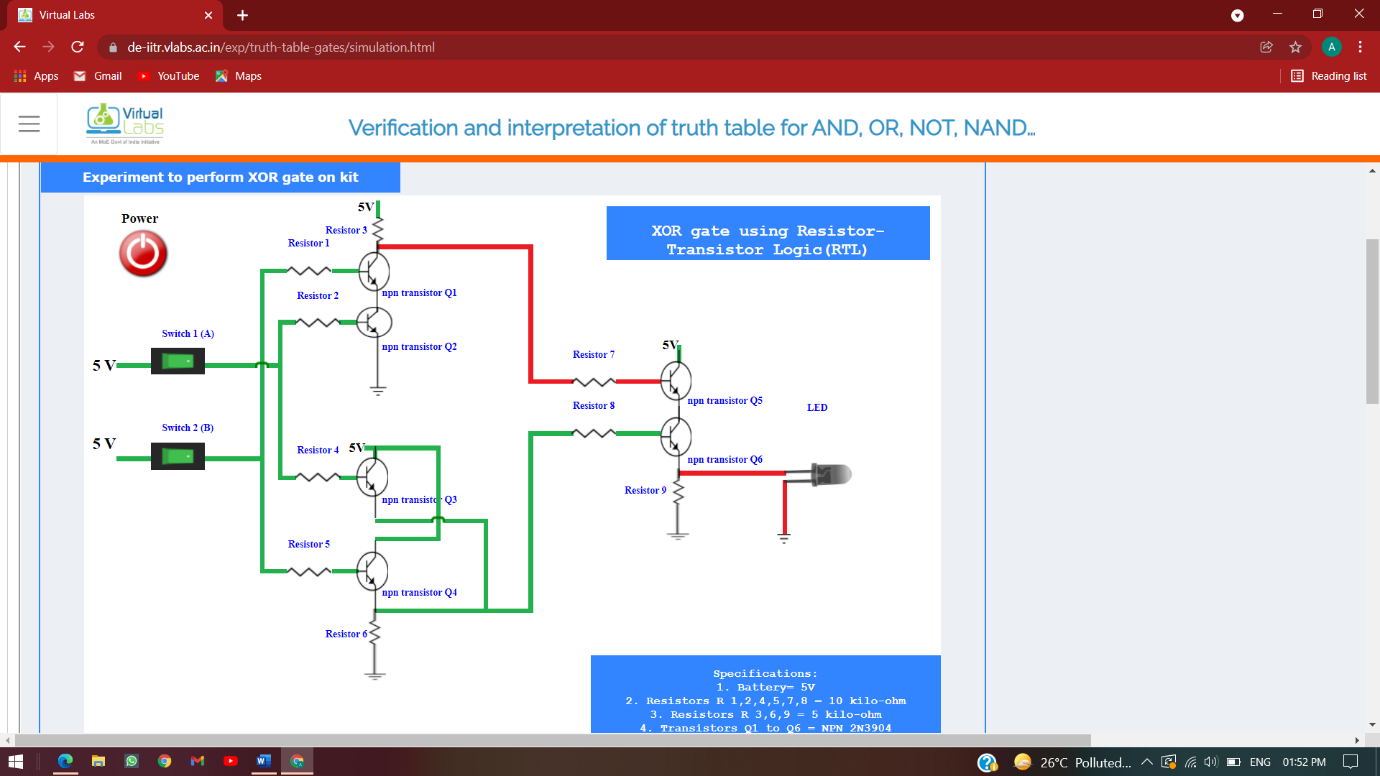
\includegraphics[width=0.9\linewidth]{img/exp6/4}
		\caption{}
		\label{fig:6:4}
	\end{figure}
		\begin{figure}[h]
		\centering
		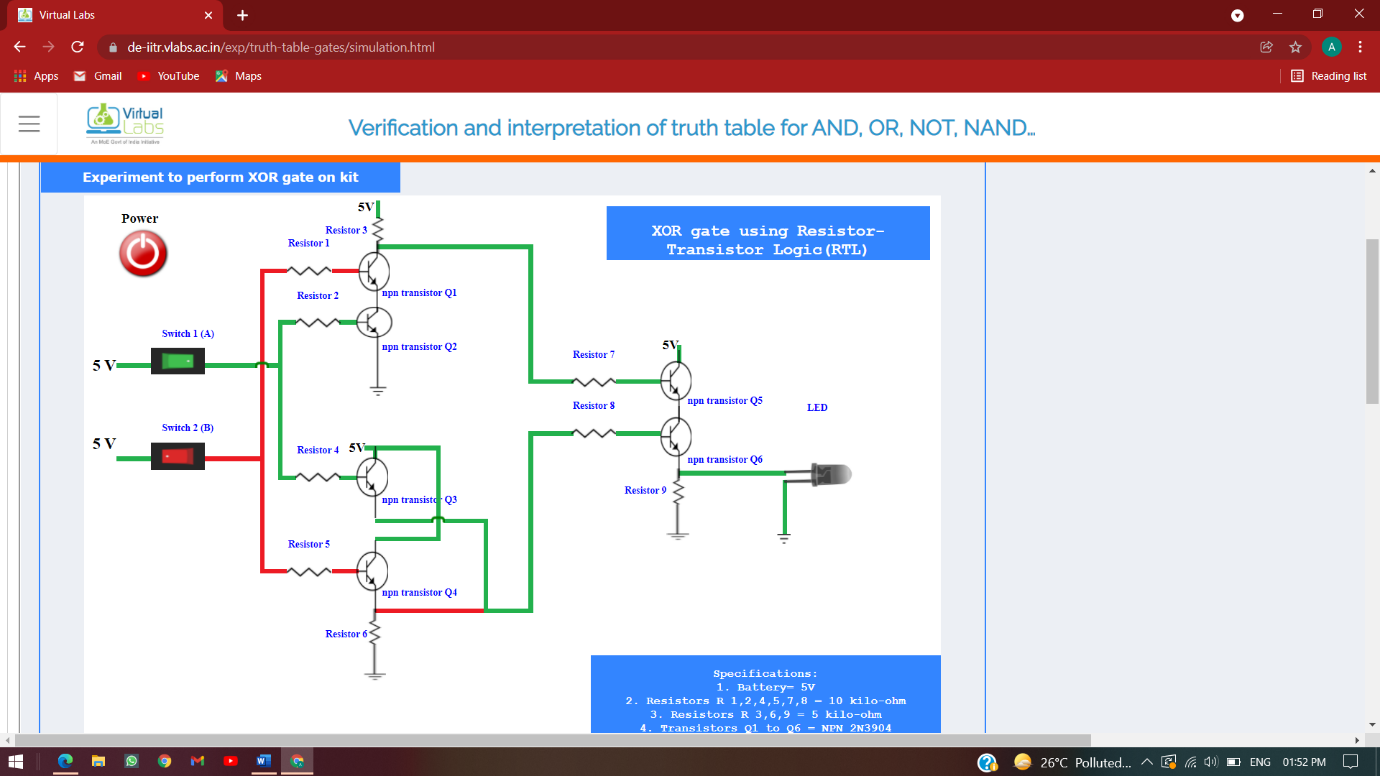
\includegraphics[width=0.9\linewidth]{img/exp6/5}
		\caption{}
		\label{fig:6:5}
	\end{figure}
		\begin{figure}[h]
		\centering
		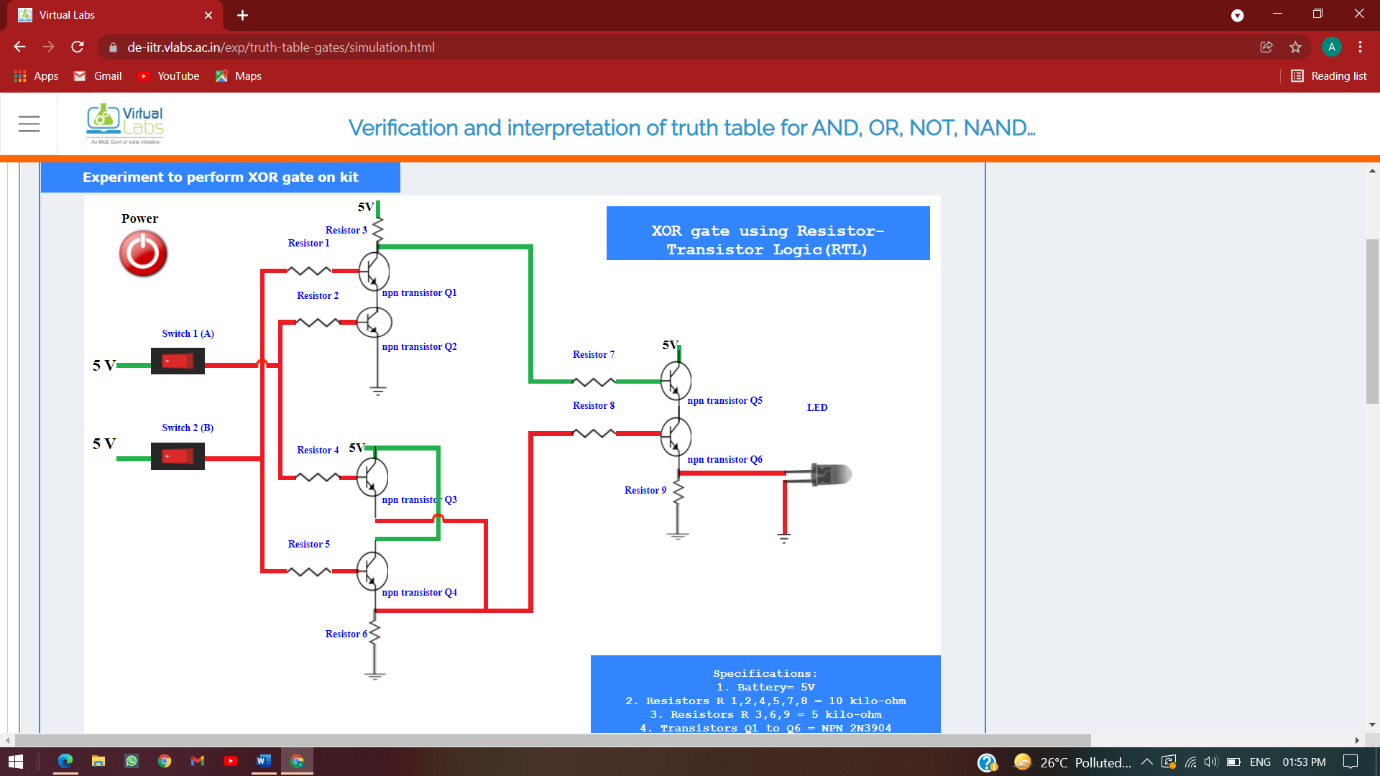
\includegraphics[width=0.9\linewidth]{img/exp6/6}
		\caption{}
		\label{fig:6:6}
	\end{figure}
		\begin{figure}[h]
		\centering
		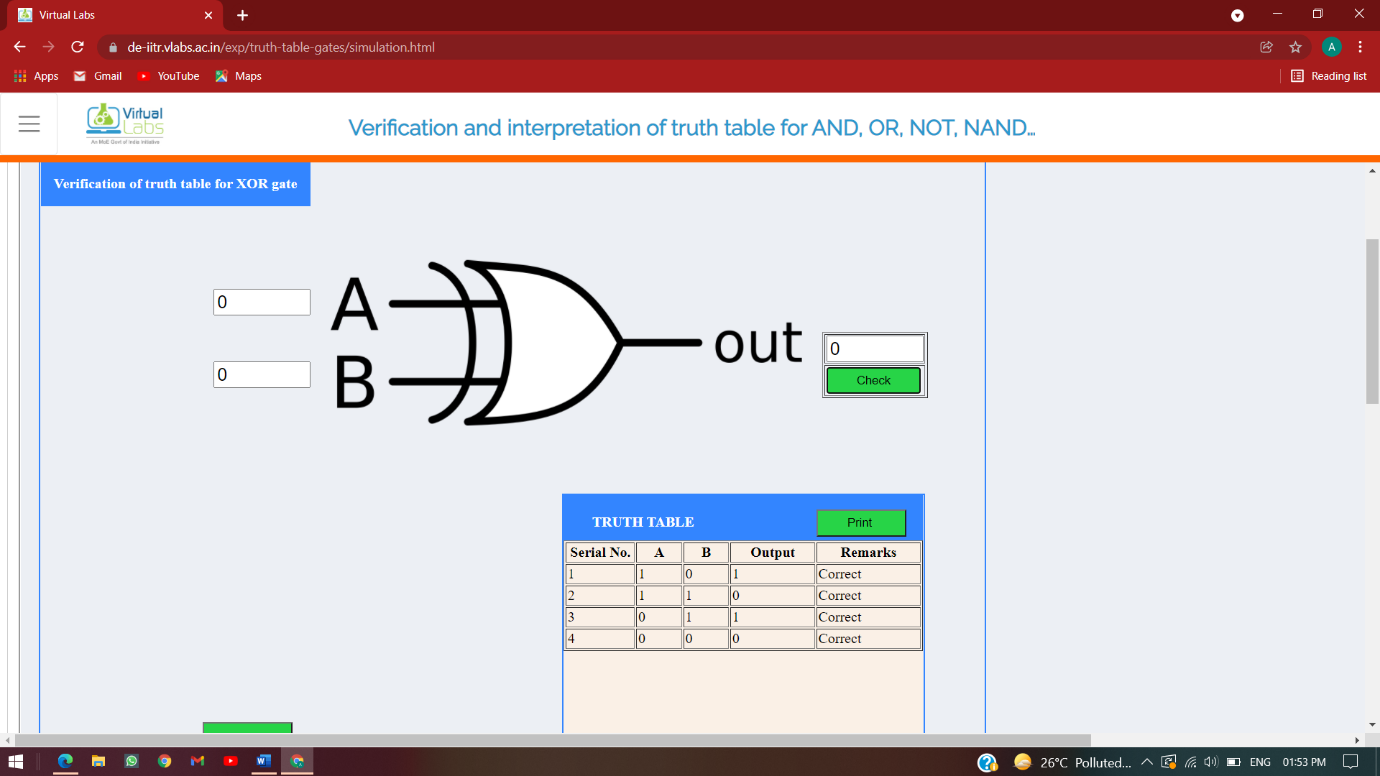
\includegraphics[width=0.9\linewidth]{img/exp6/7}
		\caption{}
		\label{fig:6:7}
	\end{figure}

\section{Conclusion}
XOR gate basically is a special version of OR gate which gives a low even when both the inputs of OR gate are high.

\section{Precautions}
	\begin{enumerate}
		\tightlist
		\item Make the connections when power supply is OFF.
		\item Ensure that the connections are tight.
		\item Change the status of inputs only when power supply is OFF.
	\end{enumerate}